\addtocontents{toc}{\protect\setcounter{tocdepth}{0}}
\section{Supplemental Figures}
\label{app:figures}
\addtocontents{toc}{\protect\setcounter{tocdepth}{1}}

\begin{figure}[h!]
    \ContinuedFloat*
    \centering
    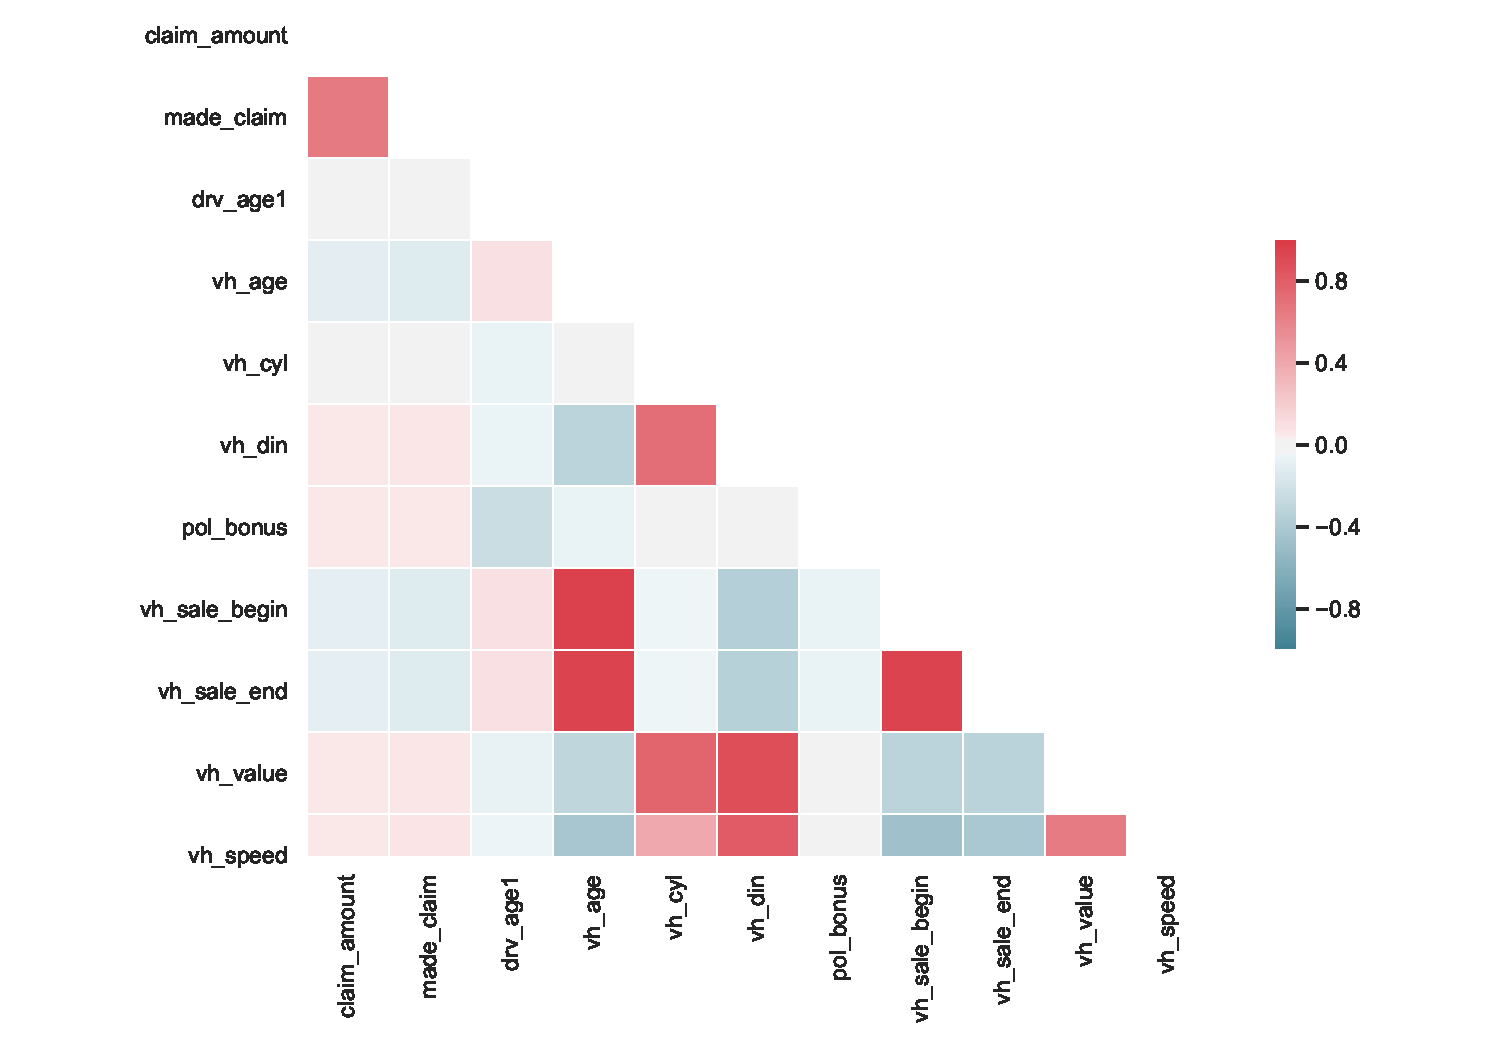
\includegraphics[width = 0.7\hsize]{./figures/corrplot.pdf}
    \caption[Correlation Matrix of Explanatory Variables]{Plot of the correlation matrix for \texttt{part2\_data.csv}. Dark red indicates a strong positive pairwise correlation between variables whereas dark blue indicates a strong negative correlation.}
    \label{fig:corrplot}
\end{figure}

\begin{figure}[h!]
    \ContinuedFloat*
    \centering
    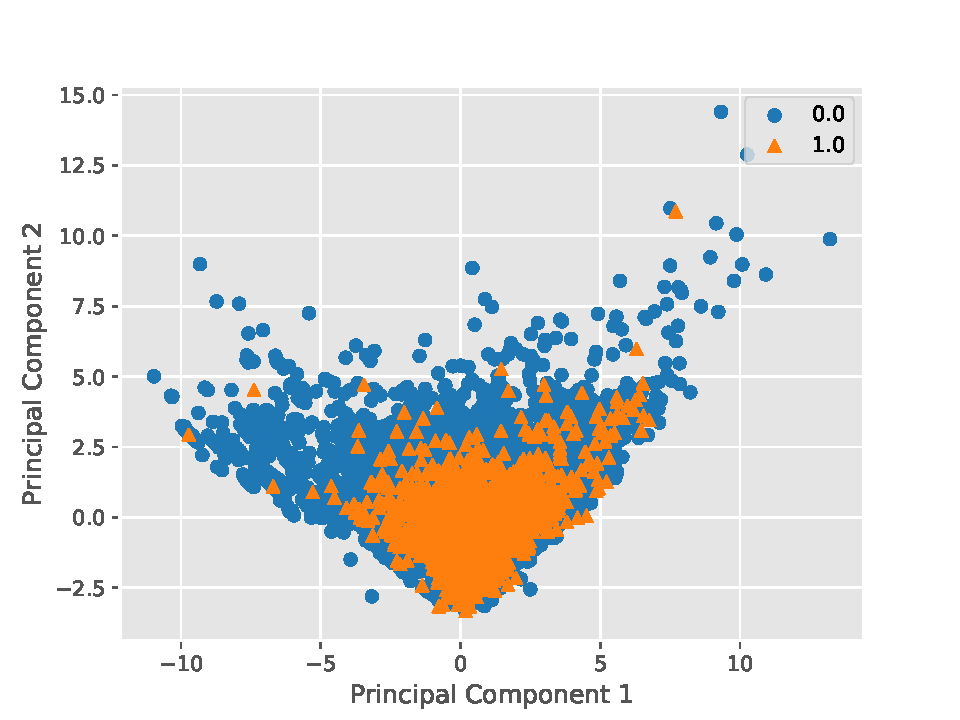
\includegraphics[width = 0.7\hsize]{./figures/pca.pdf}
    \caption[Scatter Plot of Explantory Variables post-Principal Component Analysis ($n=2$)]{Plot of \texttt{part2\_data.csv} post dimension reduction with Principal Component Analysis ($n=2$).}
    \label{fig:pca}
\end{figure}

\begin{figure}
\makebox[\linewidth][c]{%
\begin{subfigure}[b]{.6\textwidth}
    \centering
    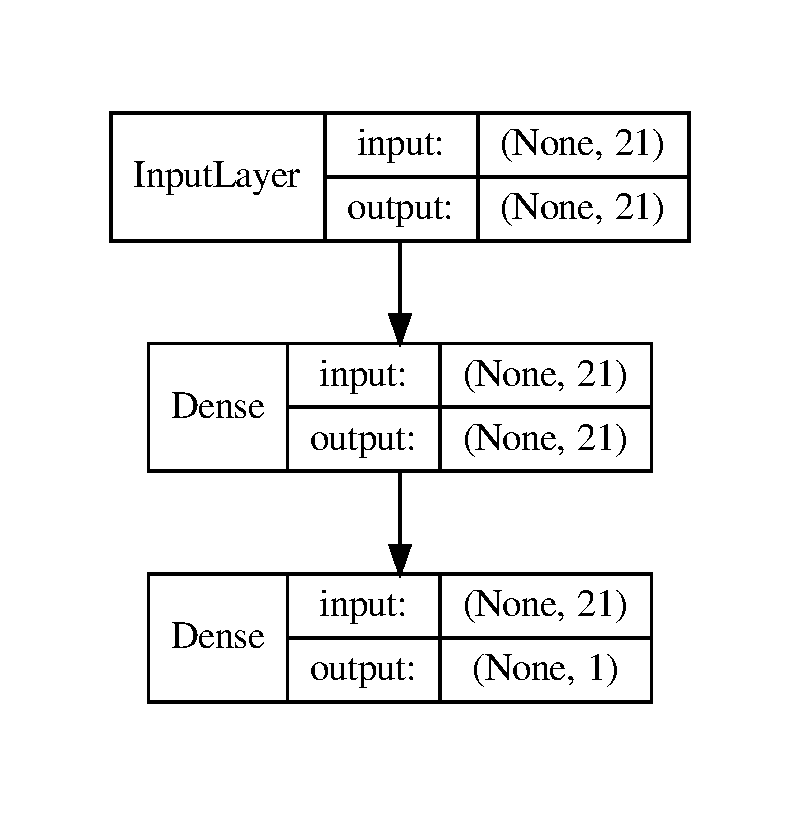
\includegraphics[width=0.8\textwidth]{figures/linear_model.pdf}
    \caption{Part 3 Linear model - Single Layer Perceptron}
    \label{fig:linmodel}
\end{subfigure}%
\begin{subfigure}[b]{.6\textwidth}
    \centering
    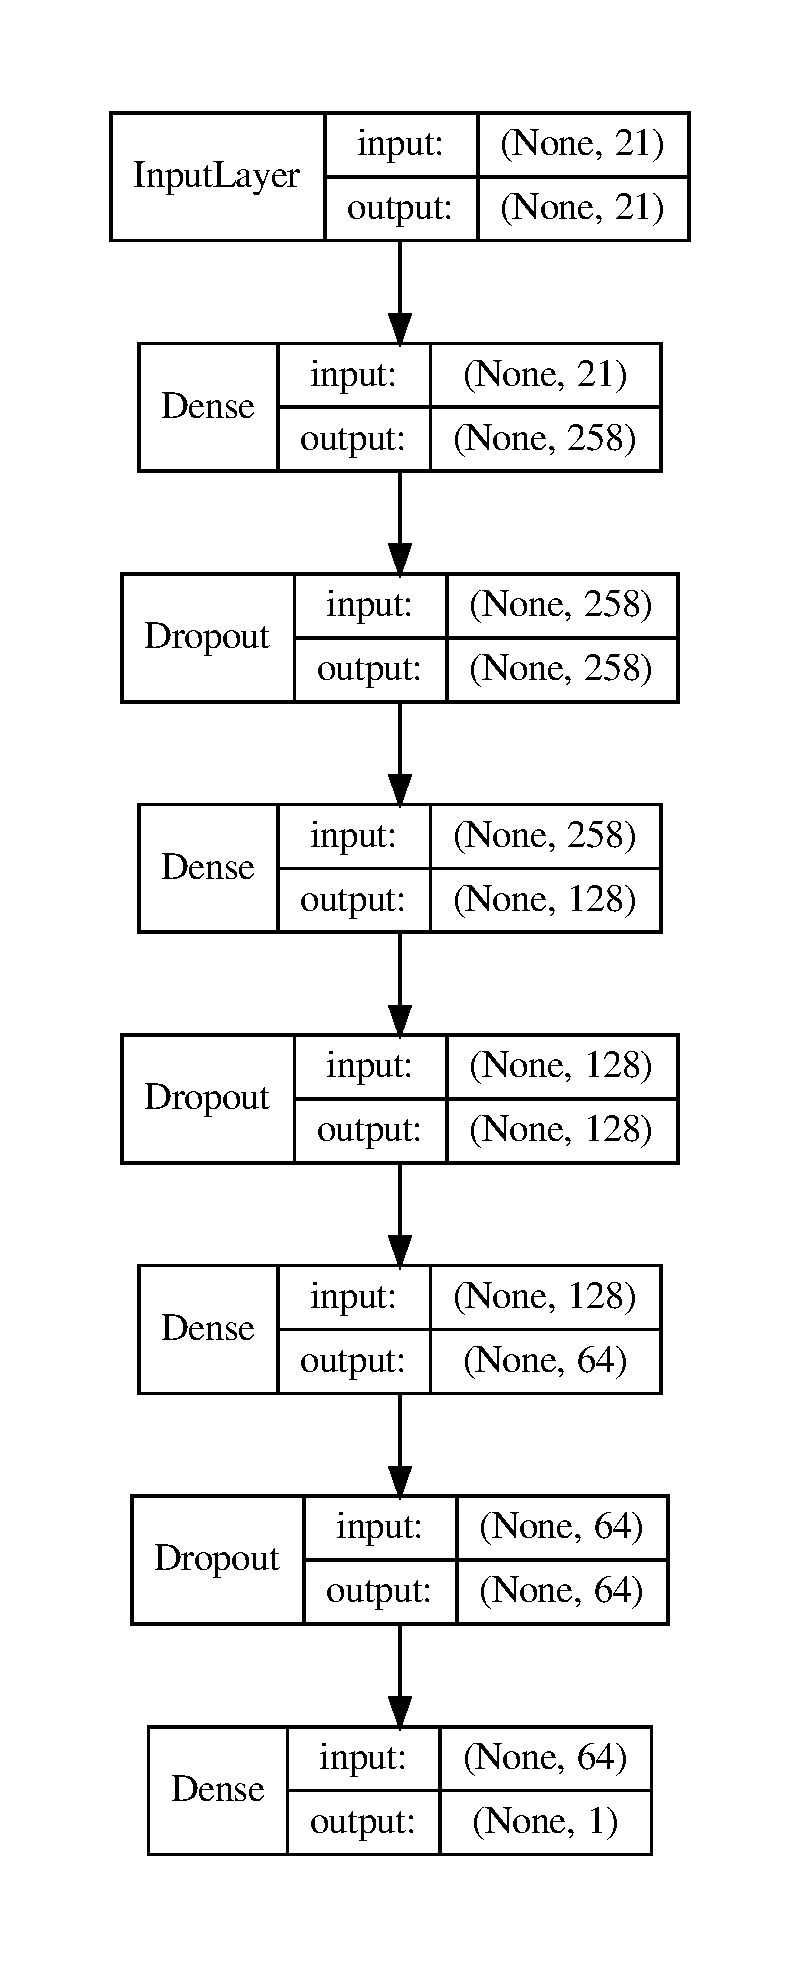
\includegraphics[width=0.8\textwidth]{figures/nonlinear_model.pdf}
    \caption{Part 3 Non Linear model.}
    \label{fig:nonlinmodel}
    \end{subfigure}%
}
\caption[Part 3 Linear and Non-linear Network Architectures]{Model Architectures}.
\label{fig:modelarchitectures}
\end{figure}